\subsection{Kommunikation}

App und Turm müssen miteinander kommunizieren. Es hätte mehrere verschiedene möglichkeiten gegeben, jedoch hat sich das Team darauf geeinigt, die bestehende Firebase Datenbank und deren "Realtime Updates" Funktion zu verwenden.

Austauschmöglichkeiten:
\begin{itemize}
  \item Websocket
  \item Firebase Cloud Messaging
  \item Firestore Datenbank Realtime Updates
\end{itemize}

\begin{figure}[H]
  \centering
  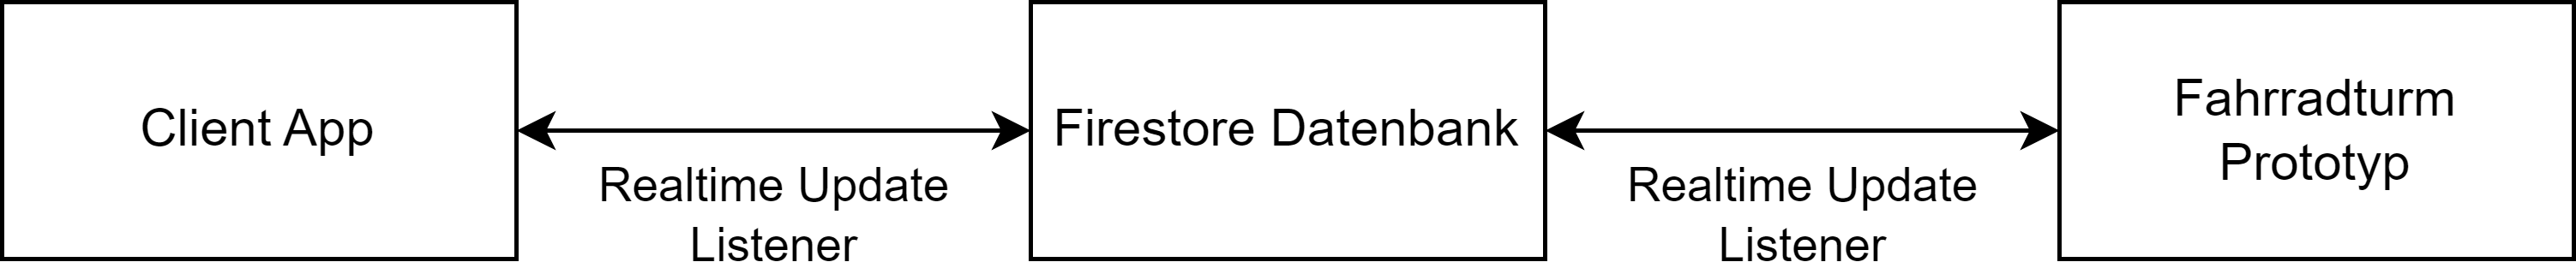
\includegraphics[width=0.9\textwidth]{images/kommunikation.png}
  \caption{Kommunikation zwischen App und Turm}
  \label{fig:kommunikation}
\end{figure}

\subsubsection{Realtime Updates}

Realtime Updates ist ein Feature von Firestore, welches es ermöglicht, dass sich Client Daten automatisch aktualisieren, sobald sich die Daten in der Datenbank ändern. Ein \Gls{listener} kann für ein oder mehrere Dokumente/Collections registriert werden und sobald sich die Daten in der Datenbank ändern, wird der \Gls{listener} automatisch über die Änderungen informiert.

\subsubsection{Fahrradturm Protokoll}

Das Fahrradturm Protokoll basiert auf Dokumenten in der Firestore Datenbank. Jedes Dokument repräsentiert einen einzelnen Job, der vom Fahrradturm ausgeführt werden soll. Die Dokumente werden in einer Subcollection des Turms namens "jobs" gespeichert. Um Jobs zu starten muss der Client ein Dokument Turms erstellen.

\paragraph{Gemeinsame Felder}

Es gibt einige Felder welche bei jedem Job vorhanden sind bzw. immer die gleiche bedeutung haben. Diese Felder sind wie folgt:

\begin{itemize}
  \item \texttt{error} ist ein optionales Feld, welches vom Fahrradturm gesetzt wird, wenn ein Fehler auftritt. Es gibt verschiedene mögliche Werte, welche die Art des Fehlers beschreiben. Anhand dieser Fehlermeldungen kann der Client die Fehlermeldung dem Nutzer anzeigen.
  \item \texttt{userId} ist die ID des Nutzers, der den Job ausführen möchte. Sie wird verwendet um festzustellen, ob der Nutzer berechtigt ist den Job auszuführen.
  \item \texttt{confirmation} ist ein optionales Feld, welches vom Fahrradturm gesetzt wird, um dem Client mitzuteilen, dass der Job erfolgreich empfangen bzw. ausgeführt wurde. Es gibt zwei mögliche Werte: \texttt{jobRecieved} und \texttt{jobCompleted}. \texttt{jobRecieved} wird gesetzt, wenn der Fahrradturm den Job empfangen hat. \texttt{jobCompleted} wird gesetzt, wenn der Fahrradturm den Job erfolgreich ausgeführt hat.
  \item \texttt{assignmentType} gibt an, welche Art von Job ausgeführt werden soll. Es gibt zwei mögliche Werte: \texttt{store} und \texttt{retrieve}.
\end{itemize}


\paragraph{Einlagern}

Einlager Jobs müssen folgende Felder enthalten:

\begin{minted}{typescript}
Job {
    assignmentType: "store",
    userId: String,
    boxType: "bike" | "item",
}
\end{minted}

\begin{itemize}
  \item \texttt{assignmentType} gibt an, dass es sich um einen Einlagerjob handelt.
  \item \texttt{boxType} gibt an, ob es sich um ein Fahrrad oder ein anderes Item handelt.
\end{itemize}

Falls der Fahrradturm den Job erfolgreich empfangen hat, wird das Feld \texttt{confirmation} auf \texttt{jobRecieved} gesetzt. Nun wird der Job auf der Seite des Fahrradturms ausgeführt. Sobald der Job abgeschlossen ist, wird das Feld \texttt{confirmation} auf \texttt{jobCompleted} gesetzt. Das Feld \texttt{boxId} wird ebenfalls gesetzt, welches die ID der Box ist, in der das Item/Fahrrad abgelegt wurde. Ein abgeschlossener Einlagerjob sieht wie folgt aus:

\begin{minted}{typescript}
Job {
    assignmentType: "store",
    userId: String,
    boxType: "bike" | "item",
    confirmation: "jobCompleted",
    boxId: String,
}
\end{minted}

\paragraph{Auslagern}

Auslager Jobs müssen folgende Felder enthalten:

\begin{minted}{typescript}
Job {
    assignmentType: "retrieve",
    userId: String,
    boxId: String,
}
\end{minted}

\begin{itemize}
  \item \texttt{assignmentType} gibt an, dass es sich um einen Auslagerjob handelt.
  \item \texttt{boxId} ist die ID der Box, aus der das Item/Fahrrad entnommen werden soll.
\end{itemize}

Ein abgeschlossener Auslagerjob sieht wie folgt aus:

\begin{minted}{typescript}
Job {
    assignmentType: "retrieve",
    userId: String,
    boxId: String,
    confirmation: "jobCompleted",
  }
\end{minted}